\PassOptionsToPackage{usenames,dvipsnames,table}{xcolor}
\documentclass[12pt,aps,preprint,nofootinbib,noshowkeys,noshowpacs,longbibliography,superscriptaddress,tightenlines]{revtex4-2}
\usepackage{amsmath,amsfonts,amsthm,amssymb}
%\usepackage{showkeys}
\usepackage{graphics,graphicx}
\usepackage[inline]{enumitem}
\usepackage{mathrsfs}
\usepackage{dsfont}
\usepackage{bm}
\usepackage{mathtools}
\usepackage{bbold}
\usepackage{xcolor}
\definecolor{darkblue}{RGB}{0,0,196}
\definecolor{darkgreen}{RGB}{0,120,0}
\usepackage{tikz}
\newcommand{\mathcolorbox}[2]{\colorbox{#1}{$\displaystyle #2$}}
\newcommand{\hlfancy}[2]{\sethlcolor{#1}\hl{#2}}
% -- highlighting
\usepackage{stackengine}
\renewcommand\useanchorwidth{T}
\newcommand\oU[1]{\ensurestackMath{\stackon[1pt]{#1}{\mkern2mu\bullet}}}
\newcommand\oX[1]{\ensurestackMath{\stackon[1pt]{#1}{\mkern2mu\star}}}
\newcommand\oY[1]{\ensurestackMath{\stackon[1pt]{#1}{\mkern2mu\smwhitestar}}}
\newcommand\oZ[1]{\ensurestackMath{\stackon[1pt]{#1}{\mkern2mu\scaleto{\circ}{3pt}}}}
\renewcommand\S{\mathcal S}
\newcommand\Sstress{{\mathcal S}}
\renewcommand\P{\mathcal P}
\newcommand\N{\mathcal N}
\newcommand\uS{{\underline{S}} }
\def\half{\tfrac{1}{2}}
\def\quarter{\tfrac{1}{4}}
\def\LF{{\scriptscriptstyle LF}}
\def\Pbb{{\mathbb P}}
\def\Ebb{{\mathbb E}}
\def\Mbb{{\mathbb M}}
\def\Sbb{{\mathbb S}}
\def\Vbb{{\mathbb V}}
\def\bbeta{{\sf b}}
\def\Teff{{\sf T}}
\newcommand{\ubeta}{{\underline{\smash{\beta}}}}
\newcommand{\uf}{{\underline{{f}}}}
\newcommand{\uu}{{\underline{u}}}
\def\pp{{\rm p}}
\def\three{{}^{(3)}}
\def\F{{\mathcal F}}
\def\K{{\mathcal K}}
\def\x{{\bm x}}
\def\p{{\bm p}}
\def\edense{{\mathcal{E}}}
\def\pdense{M}
\def\dpdense{\delta\kern-0.08em M}
\def\dbeta{\delta\kern-0.08em \beta}
\def\CChi{ {\mathcal \chi}}
\def\HP{\hphantom{\alpha}} % horizontal
\def\llangle{\left\langle}
\def\rrangle{\right\rangle}
\newcommand{\nn}{\nonumber}
\newcommand{\rl}{\mathrm{rel}}
\newcommand{\tbj}{\tau}
\newcommand{\vecxp}{\vec{x}_\perp}
\def\Pr{ {\rm p} }
\def\edense{ {\rm e} }
\def\muh{\hat\mu}
\def\vh{\hat v}
\def\noisekernel{{\kappa}}
\def\Eq#1{eq.~(\ref{#1})}
\def\Eqs#1{eqs.~(\ref{#1})}
\def\eq#1{(\ref{#1})}
\def\app#1{App.~\ref{#1}}
\def\Fig#1{Fig.~\ref{#1}}
\def\Figs#1{Figs.~\ref{#1}}
\def\Sect#1{Sect.~\ref{#1}}
\def\Ref#1{Ref.~\cite{#1}}
\def\betaz{{(\beta_0)}}


% equation environments
\def\P{\mathcal P}
\def\beq{\begin{equation}}
\def\eeq{\end{equation}}
\def\st{\begin{equation}}
\def\stp{\end{equation}}
\def\ba{\begin{eqnarray}}
\def\ea{\end{eqnarray}}
\def\DD{{\mathcal L}}
\def\vDD{{\mathcal L}}
\newcommand\vbeta{{\vec{\beta}}}
\newcommand\vcovD{D}
\newcommand\Chi{\mathcal X}
\newcommand\covD{\nabla}
\newcommand{\ve}[2]{e_{\;\,#1}^{#2}}
\newcommand{\de}[2]{e_{\;\,#2}^{#1}}
\newcommand{\vp}{{\vec{p}\,}}
\newcommand{\petsc}{{\tt PETsc}}

\def\E{{\mathcal E}}
\def\P{{\mathcal P}}
\def\M{{\mathcal M}}
\def\m{{\mathfrak m}}
\def\dd{{\rm d}}
\def\lps{{N}}
\def\sp{\phantom{j}}
\def\spm{\phantom{\mu}}
\def\sft{\vec{N}}
\def\tideal{{\mathcal T}}
\def\tvisc{\Pi}
\def\btvisc{\bar{\Pi}}
\newcommand\ph{\phantom{\nu}}

\newcommand\V{V_0}
\newcommand\dtau{{{\Delta}\tau}}
\newcommand\dt{{{\Delta}t}}

\def\bb1{{(1)}}
\def\bbt{{(2)}}
\def\bbth{{(3)}}

\newcommand{\AM}[1]{{\color{green}AM: #1}}
\newcommand{\cmtJF}[1]{{\color{blue}JF: #1}}
\newcommand{\rs}[1]{{\color{red}RS: #1}}
\newcommand{\cmtMS}[1]{{\color{cyan}MS: #1}}

\newcommand{\gammathree}{{}^{(3)}\Gamma}
\usepackage[colorlinks=true,linktocpage=true,linkcolor=darkblue,citecolor=red,urlcolor=darkblue]{hyperref}
\usepackage{newunicodechar}
\newunicodechar{Δ}{\ensuremath{\Delta}}
\usepackage{listings}
\definecolor{jlkw}{RGB}{0,0,180}
\definecolor{jlcmt}{RGB}{0,128,0}
\definecolor{jlstr}{RGB}{160,60,0}
\definecolor{jlfn}{RGB}{128,0,128}
\lstdefinelanguage{Julia}{%
  morekeywords=[1]{abstract,break,catch,const,continue,do,else,elseif,%
    end,export,false,for,function,immutable,import,if,in,%
    macro,module,mutable,return,struct,true,try,using,while,with},%
  morekeywords=[2]{zero,dot,minimum_image,wendland_c2_grad,%
    kappa_tensor,neighbors,SMatrix,rebuild_cell_list},%
  sensitive=true,%
  alsoletter={!},%
  morecomment=[l]{\#},%
  morecomment=[n]{\#=}{=\#},%
  morestring=[b]{"},%
}[keywords,comments,strings]

\lstset{
  language=Julia,
  basicstyle=\ttfamily\small,
  columns=flexible,
  keepspaces=true,
  showstringspaces=false,
  keywordstyle=[1]\color{jlkw}\bfseries,
  keywordstyle=[2]\color{jlfn},
  commentstyle=\color{jlcmt}\itshape,
  stringstyle=\color{jlstr},
  literate=
    {ε}{$\varepsilon$}{1}
    {κ}{$\kappa$}{1}
    {Δ}{$\Delta$}{1}
    {δ}{$\delta$}{1}
    {β}{$\bbeta$}{1}
    {ξ}{$\xi$}{1}
    {γ}{$\gamma$}{1}
    {η}{$\eta$}{1}
    {ζ}{$\zeta$}{1}
    {≥}{$\geq$}{1}
    {≤}{$\leq$}{1}
    {>=}{$\geq$}{2}
    {!=}{$\neq$}{2}
}

\renewcommand{\baselinestretch}{1.05}

% ============================================================================
\providecommand{\tr}{\operatorname{tr}}
\begin{document}

\title{First stochastic SPH run:\\ideal symplectic step $+$ per-particle Metropolis sweep}
\author{D.~Teaney}
\affiliation{Department of Physics and Astronomy, Stony Brook University,
Stony Brook, New York 11794, USA}
\date{\today}

\begin{abstract}
Working notes for the first stochastic SPH run.  One deterministic \emph{ideal}
symplectic step is followed by a single Metropolis sweep over the
\emph{particles}.  Each particle move draws one Gaussian stress $\xi_a$ at particle
$a$, applies it as momentum- and energy-conserving kicks through \emph{all} of
$a$'s bonds, and is accepted with $\min(1,e^{\Delta\Sbb_a})$, where
$\Delta\Sbb_a = \Delta t\,V_a\,\xi_a\!:\!\varepsilon_a$ sees the full SPH
strain.  \emph{All} dissipation comes from the accept/reject asymmetry; there
is no separate deterministic dissipative step.  The mean drift of the sweep is
\emph{exactly} the deployed two-level viscous force
\texttt{dissipative\_force!}, and the noise covariance is forced by the match
--- there is no free amplitude and nothing to calibrate.  Derivations,
accuracy limits, and the implementation plan are collected in the appendices;
the end target is the stochastic decay of a 2D sound wave.
\end{abstract}

\maketitle
\tableofcontents

% ============================================================================
\section{Scope and notation}
\label{sec:scope}

Notation follows \texttt{sph2.tex}: particle $a$ carries the extensive entropy
$s_a$ and momentum $m_a^i$; the smoothed entropy field is
$S(x_a)=\sum_b s_b W(x_a,x_b)$; the EOS solve yields $v_a$, $\gamma_a$,
$T_{{\rm rel},a}$; and the smoothed conjugates give the velocity $\dot x_a$,
the temperature $\Teff_a$, and
\st
\bbeta_a \equiv \frac{\dot x_a}{\Teff_a}\,.
\stp
$D_j(x_a,x_b)\equiv\partial W(x_a,x_b)/\partial x_a^j$ is the kernel gradient,
with $D_j(x_b,x_a)=-D_j(x_a,x_b)$, and $V_a\equiv s_a/S_a$ is the particle
``volume'' (the SPH estimate of $\dd^dx$, \texttt{sph2.tex} App.~D).

Three results from \texttt{sph2.tex} are used verbatim :
\begin{itemize}
  \item Density-frame noise covariance (FDT):
        \st
        \label{eq:fdt}
        \llangle \xi^{ij}(\x,t)\,\xi^{lm}(\x',t')\rrangle
          = 2\,T_{\rm rel}\,\kappa^{ijlm}(v)\;\delta(t-t')\,\delta^2(\x-\x')\,.
        \stp
  \item Tthe entropy change that keeps $\mathbb H$ fixed
        under a momentum kick $\Delta m_a$ (to linear order;
        \app{app:accuracy}):
        \st
        \label{eq:ds}
        \Delta s_a = -\,\bbeta_a\cdot\Delta m_a\,.
        \stp
  \item Total entropy change:
        \st
        \label{eq:dS}
        \Delta\Sbb = \sum_a \Delta s_a = -\sum_a \bbeta_a\cdot\Delta m_a\,.
        \stp
\end{itemize}


For deterministic hydro  the viscous force was computed in two passes
(\texttt{sph2.tex} App.~D,    \texttt{dissipative\_force!}): Pass~1 builds the
SPH strain
\st
\label{eq:strain}
\varepsilon_{ji}(x_a) \;=\; \frac{1}{S(x_a)}\sum_b s_b\,
   \big(\bbeta_{i,b}-\bbeta_{i,a}\big)\,D_j(x_a,x_b)
\stp
and Pass~2 assembles the viscous force
\st
\label{eq:twolevel}
f^i_{\rm det}(x_a) = \sum_b s_a s_b\,D_j(x_a,x_b)
    \left[\frac{T_{\rm rel}\kappa^{ijlm}}{S^2}\bigg|_a\varepsilon_{lm}(x_a)
        + \frac{T_{\rm rel}\kappa^{ijlm}}{S^2}\bigg|_b\varepsilon_{lm}(x_b)\right].
\stp
We will show how the stochastic step reproduces this mean strain

% ============================================================================
\section{The stochastic step}
\label{sec:step}

A full step takes $(x_a^n,m_a^n,s_a^n)\to(x_a^{n+1},m_a^{n+1},s_a^{n+1})$ by
an ideal sub-step followed by one per-particle sweep.

\paragraph{A --- ideal symplectic sub-step.}
Advance $(x_a,m_a)$ by one step of the \emph{ideal} Hamiltonian flow with the
2nd-order symplectic integrator at fixed $\Delta t$ (acoustic CFL).  No
dissipative or stochastic term here: $s_a$ is unchanged and $\Sbb$,
$\mathbb H$ are conserved to integrator order.

\paragraph{B --- freeze and strain.}
Freeze a snapshot of the coefficients
$\{S_a, s_a, \bbeta_a, v_a, \gamma_a, T_{{\rm rel},a}, \kappa|_a\}$ and
precompute the strain $\varepsilon_a$ \eqref{eq:strain} at every particle.
During the sweep only the accumulated increments $(\Delta m_a,\Delta s_a)$
change; they are applied to $(m_a,s_a)$ once, at the end of the sweep, and the
coefficients are then refreshed for the next step.

\paragraph{C --- the proposal at particle $a$.}
For particle $a$, draw one symmetric $2\times2$ Gaussian stress
$\xi_a^{ij}=\xi_a^{ji}$, mean zero, with covariance
\st
\label{eq:persite_cov}
\boxed{\;
\llangle \xi_a^{ij}\,\xi_a^{lm}\rrangle
   \;=\; \frac{2\,T_{{\rm rel},a}\,\kappa^{ijlm}(v_a)}{\Delta t\,V_a}\,,
\qquad V_a \equiv \frac{s_a}{S_a}\;}
\stp
This is the discretised FDT \eqref{eq:fdt} with $\delta(t)\to1/\Delta t$ and
$\delta^d(x)\to1/V_a$.  From $\xi_a$ build a \emph{proposal}: a trial update
of $a$ and all of its neighbours, patterned on the particle-$a$ stress piece of
the viscous force \eqref{eq:twolevel}.  The proposed momentum changes are,
for every bond $(a,b)$ with $r_{ab}<2h$,
\st
\label{eq:kicks}
\boxed{\;
\Delta m_a \mathrel{+}= \Delta t\,\frac{s_a s_b}{S_a^{2}}\,\xi_a^{ij}D_j(x_a,x_b)\,,
\qquad
\Delta m_b \mathrel{-}= \Delta t\,\frac{s_a s_b}{S_a^{2}}\,\xi_a^{ij}D_j(x_a,x_b)\,,\;}
\stp
together with $\Delta s_c=-\bbeta_c\cdot\Delta m_c$ \eqref{eq:ds}, for every
particle $c$ neighboring $a$.  The proposal conserves
momentum bond by bond, conserves $\mathbb H$ to linear order in the kick, and
has $\Delta m\sim\sqrt{\Delta t}$; positions are untouched.  Nothing is
applied yet --- whether the trial update is kept is decided next.

\paragraph{D --- accept / reject.}
The entropy change of the proposed update collapses onto the strain:
\begin{align}
\Delta\Sbb_a
  &= \sum_c \Delta s_c \\
  &= -\sum_c \bbeta_c\cdot\Delta m_c
   = \Delta t\,\frac{s_a}{S_a^{2}}\,\xi_a^{ij}
     \sum_b s_b\big(\bbeta_{i,b}-\bbeta_{i,a}\big)D_j(x_a,x_b) \nn\\[2pt]
  &= \boxed{\;\Delta t\;V_a\;\xi_a^{ij}\,\varepsilon_{ji}(x_a)\;}
\label{eq:dSa}
\end{align}
This is the discrete form of $\int\!\dd t\,\dd^d x\;\xi^{ij}\partial_j\beta_i$,
and of either sign.  Note to compute $\Delta \Sbb_a$ at this linearized level we can just the previously stored strain.  Accept the proposal with probability
\st
\boxed{\;
P_{\rm acc}(a) = \min\!\big(1,\ e^{\,\Delta\Sbb_a}\big)\,;
\;}
\stp
on acceptance the trial $(\Delta m,\Delta s)$ are added to the accumulators;
on rejection the proposal is discarded entirely and the state is unchanged.
Because
$\xi_a\to-\xi_a$ is equiprobable and the covariance depends only on frozen
coefficients, this is a plain symmetric-proposal Metropolis move: it preserves
the target weight $\propto e^{\Sbb}$ on the $(\mathbb H,\mathbf P)$ level set
fixed by the ideal flow.  Dissipation is entirely the acceptance asymmetry.

\paragraph{E --- the sweep.}
Zero the increment accumulators $(\Delta m_a,\Delta s_a)$, then one pass over
all particles $a=1\dots N$, each visited once, accumulating accepted kicks;
then fold the accumulators into $(m_a,s_a)$ and refresh.  With the freeze the
moves are mutually independent, so the sweep is order-free and parallel
(\app{app:sweep}).  Exactly one sweep per ideal step: the covariance
\eqref{eq:persite_cov} carries the $\Delta t$.

% ============================================================================
\section{Mean drift}
\label{sec:det}

$\Delta m$ and $\Delta\Sbb_a$ are both linear in the Gaussian $\xi_a$, so the
Metropolis average follows from the identity
$\llangle X\min(1,e^{Y})\rrangle=\tfrac12\llangle XY\rrangle+O(\sigma^3)$ for
mean-zero jointly Gaussian $(X,Y)$.  Applied to a single particle move, and summing the
sweep --- particle $a$ is kicked once by its \emph{own} move (the particle-$a$
stress term) and once, in reaction, by \emph{each neighbour's} move (their
particle-$b$ stress terms; the draws are independent, so the means add) --- the
result is (\app{app:drift})
\st
\label{eq:drift_full}
\boxed{\;
\big\langle\Delta m_a\big\rangle_{\rm acc}
  = \Delta t\sum_b s_a s_b\,D_j(x_a,x_b)
    \left[\frac{T_{\rm rel}\kappa^{ijlm}}{S^2}\bigg|_a\varepsilon_{lm}(x_a)
        + \frac{T_{\rm rel}\kappa^{ijlm}}{S^2}\bigg|_b\varepsilon_{lm}(x_b)\right]
  = \Delta t\,f^i_{\rm det}(x_a)\,,\;}
\stp
the \textbf{full} two-level force \eqref{eq:twolevel}.  Two cancellations in
the derivation are structural: the Metropolis $\tfrac12$ (only the downhill
half of the noise is suppressed) exactly eats the FDT factor of~$2$ in
\eqref{eq:persite_cov}, and the $1/V_a$ from the discretised $\delta^d(x)$
supplies the volume power that a naive per-bond force misses
(\app{app:perbond}).  The covariance \eqref{eq:persite_cov} is therefore
\emph{forced} by the match: there is no free amplitude, and the shear-wave and
sound-wave runs are \emph{validations}, not calibrations.

% ============================================================================
\section{Diagnostics --- what ``working'' means}
\label{sec:checks}

\begin{itemize}
  \item \textbf{Momentum:} $\sum_a m_a^i$ constant to machine precision.
  \item \textbf{Energy:} $\mathbb H$ shows the \emph{expected} small positive
        drift at relative rate $\sim1/(s_a\tau_{\rm visc})$
        [\app{app:accuracy}] on top of the integrator error --- linear in $t$,
        with the predicted magnitude; anything faster is a bug.
  \item \textbf{Second law:} $\langle\Delta\Sbb\rangle\ge0$ per sweep;
        individual moves go both ways.
  \item \textbf{Acceptance:} near unity ($\gtrsim0.99$) in the small-kick
        regime; it is \emph{not} tuned.  Low acceptance means $\Delta t$ is
        too large for the given $\eta/s$ and gradients.
  \item \textbf{Grid-scale modes:} $\mathrm{rms}(m_a)$ on a quiescent uniform
        background must \emph{saturate} at the FDT equipartition value
        ($\langle v_a^2\rangle\sim1/s_a$; requires $s_a\gtrsim10^3$ for
        non-relativistic thermal fluctuations), in contrast to the per-bond
        $\sqrt t$ runaway (\app{app:perbond}).
  \item \textbf{Equilibrium fluctuations:} time-averaged
        $\langle\delta S^2\rangle$, $\langle m^2\rangle$ vs.\ the FD
        prediction; repeat at $\Delta t/2$ to bound the $O(\Delta t)$ weak
        bias [\app{app:accuracy}].
  \item \textbf{Mean drift:} sweep-averaged $\Delta m_a/\Delta t$ on a frozen
        sheared state matches \texttt{dissipative\_force!} ---
        \eqref{eq:drift_full} head-to-head.
  \item \textbf{Shear wave (validation):} decay rate of $M^y=A\sin(kx)$
        matches $\gamma_k=(\eta/s)\,k^2/T_0$ with no tuned parameter.
  \item \textbf{$\eta/s\to0$:} $\xi_a\to0$; the run reduces to the
        deterministic ideal symplectic integrator.
\end{itemize}

% ============================================================================
\section{First results on a frozen lattice}
\label{sec:results}

The unit checks of \texttt{teststochastic.jl} all pass: momentum is conserved
to round-off, the sweep is visit-order independent, and the mean drift of the
sweep reproduces \texttt{dissipative\_force!} (slope $0.994\pm0.007$).  The
uniform-background run \texttt{examples/teststochastic\_run.jl}, however,
fails.  Started at the FDT equilibrium with the ideal step on, after 3000
steps $\mathrm{rms}(M)$ is $157$ times the FDT value and $\mathbb H$ has
grown by $115\%$.  (Before the cell-list fix described below it blew up at
step 419.)  This section isolates why, with the particles held fixed so that
only the stochastic sweep acts.

\paragraph{Setup (all figures).}
2D conformal fluid, $c_s^2=1/2$, units $\ell_Q=T_0=1$, $s_0=1$,
$\eta/s=10/\sqrt2\approx7.07$, $\zeta=0$.  Hex lattice with $h=15$, $h/a=2.55$
($a=5.88$), box $147.1\times152.8$, $N=750$, particle volume $V=29.97$,
$s_a\approx30$, $T_{\rm rel}=0.912$, $w=e+p=0.759$; each particle has 91
neighbours within $2h$.  $\Delta t=4.24$ (acoustic CFL $0.2$) unless stated.
\emph{Frozen lattice} means no ideal step: positions never move, and each step
is refresh fields $\to$ \texttt{particle\_sweep!} $\to$ \texttt{apply\_sweep!}.
\emph{Cold start} means all $m_a=0$ initially: all of the energy is internal,
none kinetic.  The scripts are in \texttt{examples/} and named in each caption.

\paragraph{A cell-list bug, now fixed.}
Drawing the cells (\Fig{fig:cold}) exposed a bug in \texttt{CellList2D}: it
used one square cell width $L_x/n_x$ in both directions.  In this box
$L_y/n_y<L_x/n_x$, so the rows of cells did not tile $[0,L_y)$, the periodic
$y$-stencil did not connect the top and bottom rows, and $5\%$ of the
neighbour pairs (all across $y=0$) were dropped; $S(x_a)$ fell to $0.83$
there on a uniform lattice.  The cells now have separate widths
$(L_x/n_x,\,L_y/n_y)$; \texttt{test/testcelllist\_box.jl} checks this.  All
results below are with the fix.  The fix changes the numbers by $\sim20\%$ but
neither of the two problems below.

% ----------------------------------------------------------------------------
\subsection{Cold start: what the sweep does to particles at rest}

\begin{figure}[t]
\centering
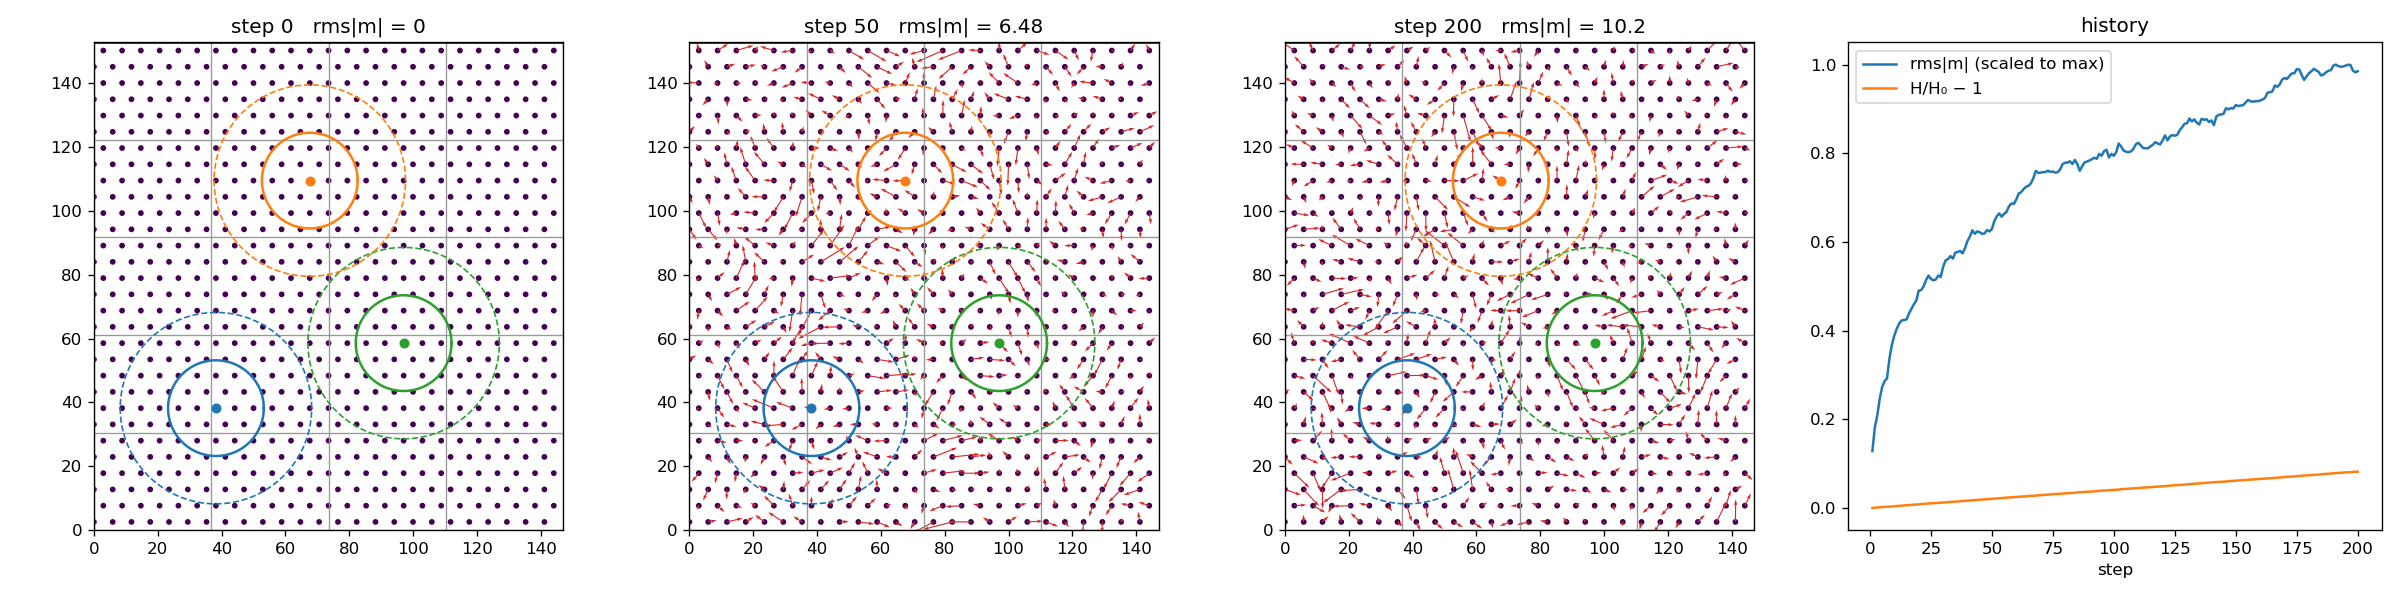
\includegraphics[width=\textwidth]{figs/simple_cold_start.png}
\caption{Cold start, frozen lattice (\texttt{simple\_cold\_start.jl}).
Panels 1--3: particles at steps 0, 50, 200; arrows are $m_a$ (rescaled per
panel, so compare the rms values in the titles, not arrow lengths).  Dots are
coloured by $S(x_a)$, uniform as it should be.  Grey lines: cell-list cells.
Circles of radius $h$ (solid) and $2h$ (dashed, the kernel support) around
three particles.  Panel 4: $\mathrm{rms}|m|$ (scaled to its maximum) and
$\mathbb H/\mathbb H_0-1$ vs step.}
\label{fig:cold}
\end{figure}

\Fig{fig:cold} is the most basic run.  The noise immediately builds a momentum
field that changes direction from one particle to the next, on the lattice
spacing $a$, which is much shorter than $h$.  Inside a single $h$-circle (about
20 particles) the arrows point every which way, so the smoothed field
$M(x)=\sum_b m_b W(x-x_b)$ averages most of this momentum away.
$\mathrm{rms}|m|$ is $6.5$ at step 50 and $10.2$ at step 200 and is still
rising.  A working scheme would saturate at the FDT value.  $\mathbb H$ rises
in a straight line ($+8.2\%$ by step 200).  With $\mathbb H$ fixed, the
fluctuation kinetic energy should instead come \emph{out} of the internal
energy: by equipartition about $T$ per particle against $s_aT\approx30T$
internal, a few percent of $\mathbb H$.

% ----------------------------------------------------------------------------
\subsection{The failures do not go away as $\Delta t\to0$}

\begin{figure}[t]
\centering
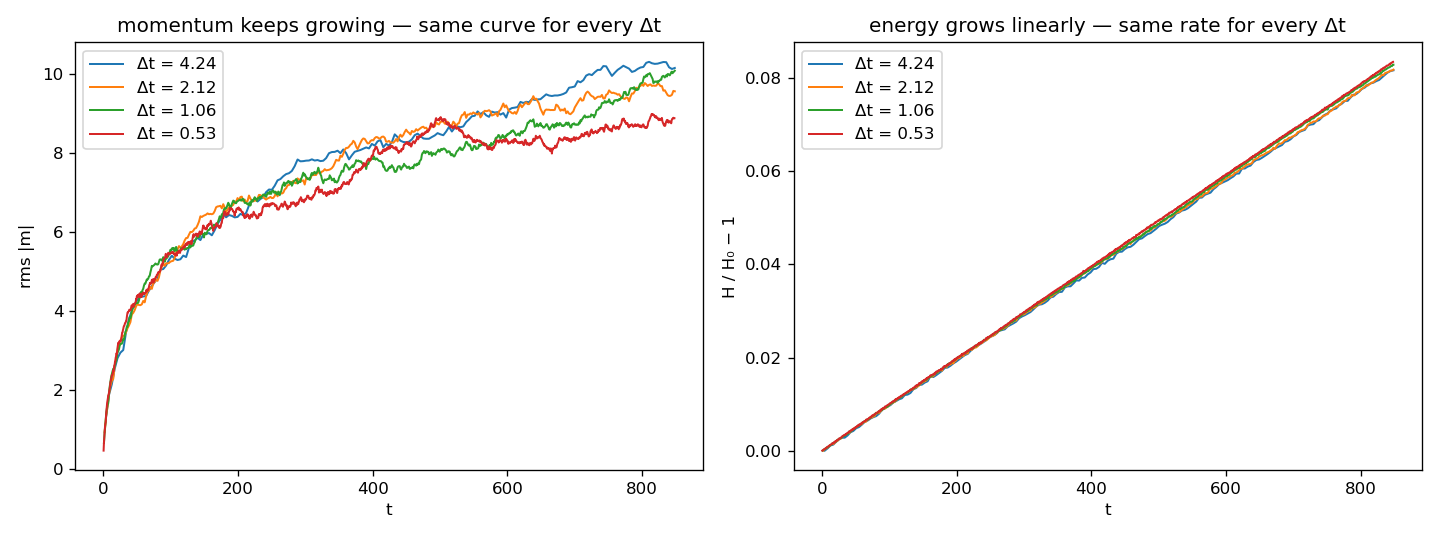
\includegraphics[width=0.9\textwidth]{figs/dt_scan.png}
\caption{Cold start, frozen lattice, four time steps run to the same physical
time $t\approx848$ (\texttt{dt\_scan.jl}).  Left: $\mathrm{rms}|m|$.
Right: $\mathbb H/\mathbb H_0-1$.}
\label{fig:dt}
\end{figure}

\Fig{fig:dt} repeats the cold start at $\Delta t=4.24,\,2.12,\,1.06,\,0.53$,
always to the same physical time.  The curves lie on top of each other (at
$t\approx848$: $\mathrm{rms}|m|=10.2,\,9.6,\,10.1,\,8.9$ and
$\mathbb H/\mathbb H_0-1=0.082,\,0.082,\,0.083,\,0.084$), and the acceptance
goes to 1 as $\Delta t\to0$ ($0.961\to0.986$).  The scheme is converging to a
well-defined continuous-time limit; it is that limit that is wrong.  The
$O(\Delta t)$ weak biases of \app{app:accuracy}(a) would shrink, so these are
not them.  Two separate defects:
\begin{enumerate}
  \item \textbf{Energy.}  $\mathbb H$ grows at $\approx1.0\times10^{-4}$ per
        unit time, independent of $\Delta t$.  This is the linearized
        $\Delta s=-\bbeta\cdot\Delta m$ of \app{app:accuracy}(b).  The dropped
        term $\tfrac12\Delta m\cdot\partial^2\mathbb H\cdot\Delta m$ is
        $O(\Delta t)$ per step and always positive, so it adds up to an $O(1)$
        drift in physical time.  It is suppressed by $1/s_a$, and $s_a=30$
        here is not large.
  \item \textbf{Momentum.}  $\mathrm{rms}|m|$ keeps growing in the
        continuous-time limit.  The rest of this section shows why.
\end{enumerate}

% ----------------------------------------------------------------------------
\subsection{What the smoothing sees: the response $R(k)$}

\begin{figure}[t]
\centering
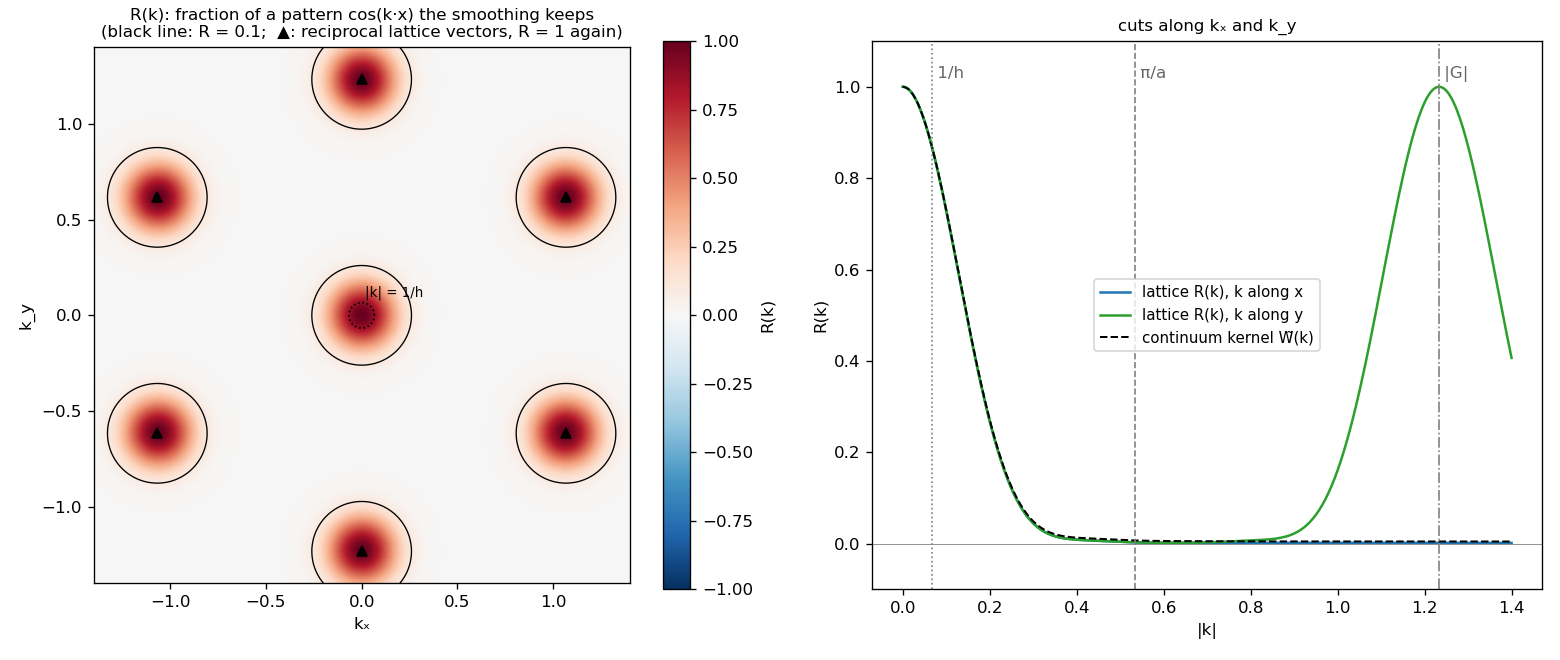
\includegraphics[width=0.95\textwidth]{figs/smoothing_response.png}
\caption{Smoothing response of the lattice (\texttt{smoothing\_response.jl}).
Left: $R(\mathbf k)$ in the plane; black contour $R=0.1$; dotted circle
$|k|=1/h$; triangles: reciprocal lattice vectors (copies of $k=0$).
Right: cuts along $k_x$ and $k_y$ compared with the continuum kernel
transform $\tilde W(k)$.}
\label{fig:R}
\end{figure}

Everything in the scheme ($\mathbb H$, $\dot x$, $\bbeta$, the strain, the
accept test) sees the particle momenta only through $M(x_a)$.  Put a wave on
the particles, $m_b=\hat m\cos(\mathbf k\cdot\mathbf x_b)$.  Converted back to a
momentum per particle, the smoothed field returns it scaled:
\st
V\,M(x_a) = R(\mathbf k)\,\hat m\cos(\mathbf k\cdot\mathbf x_a)\,,\qquad
R(\mathbf k) = V\sum_b W(x_a-x_b)\cos\!\big(\mathbf k\cdot(\mathbf x_b-\mathbf x_a)\big)\,.
\label{eq:R}
\stp
$R(\mathbf k)$ is the fraction of the wave the smoothed field keeps.
\Fig{fig:R} evaluates \eqref{eq:R} on the actual neighbours.  $R(0)=1.0002$
(a uniform flow is fully seen), and the lattice sum matches the continuum
$\tilde W(k)$ up to $|k|\approx1$.  $R$ falls to $0.5$ at $|k|\approx0.15$, to
$0.1$ at $|k|\approx0.26$, and is essentially zero beyond $|k|\approx0.35$
(a wavelength of about $1.2h$).  On a lattice, $\mathbf k$ and
$\mathbf k+\mathbf G$ give the same pattern, which is why $R$ returns to 1 at
the reciprocal vectors ($|G|=4\pi/\sqrt3a=1.23$).  Every distinct pattern has
a $\mathbf k$ in one hexagonal zone of area $\approx1.32$, and $R>0.1$ only in a
disk of area $\approx0.21$.  So \textbf{only about $16\%$ of the lattice's
momentum patterns are seen by the smoothing at more than $10\%$}.  This is the
price of $h/a=2.55$: each smoothed value averages over about 90 neighbours.

% ----------------------------------------------------------------------------
\subsection{The growing momentum is the part the smoothing does not see}

\begin{figure}[t]
\centering
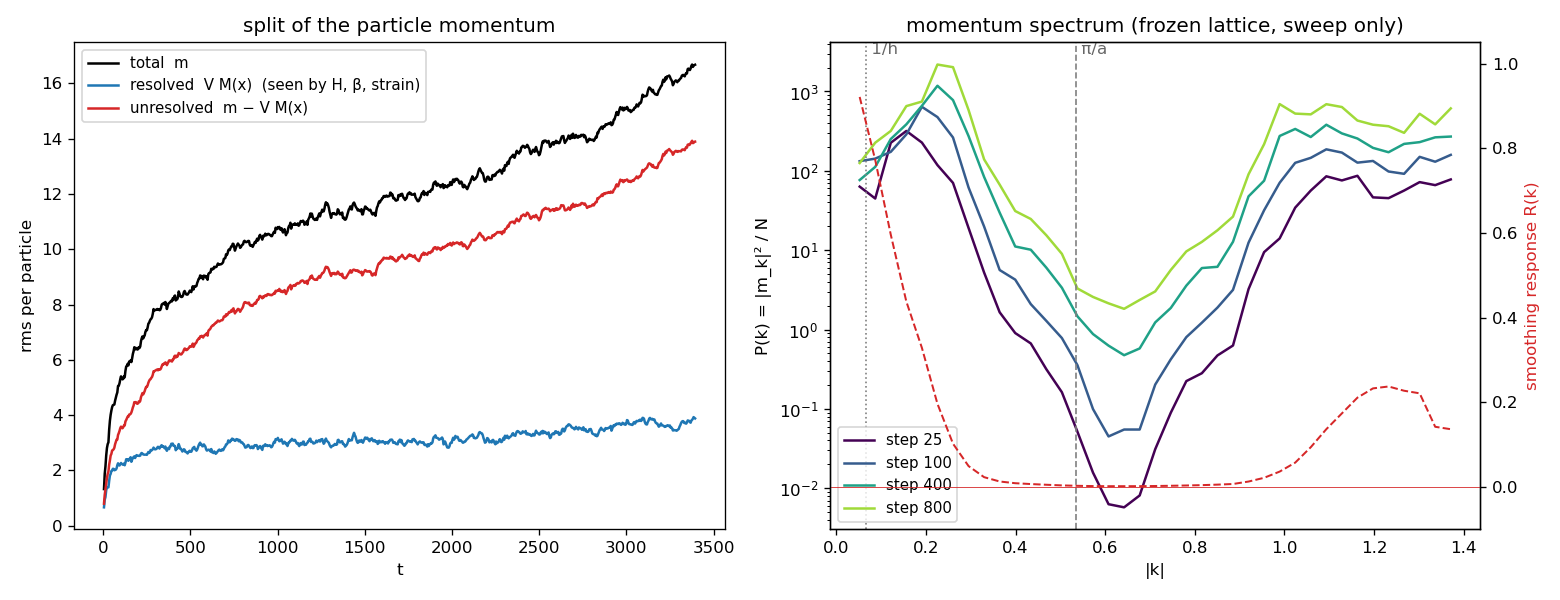
\includegraphics[width=\textwidth]{figs/momentum_split.png}
\caption{Cold start, frozen lattice, 800 steps (\texttt{momentum\_split.jl}).
Left: rms of the total momentum, its resolved part $V_aM(x_a)$ and its
unresolved part $m_a-V_aM(x_a)$.  Right: spectrum
$P(\mathbf k)=|\sum_a m_a e^{-i\mathbf k\cdot\mathbf x_a}|^2/N$ binned in $|k|$
at four times, with $R$ (red dashed, right axis) averaged in the same bins.
The bump at $|k|>1$ is lattice aliasing of the low-$k$ modes (\Fig{fig:R}).}
\label{fig:split}
\end{figure}

Split each particle's momentum into the part the smoothed field sees and the
rest:
\st
m_a = \underbrace{V_a M(x_a)}_{\rm resolved}
    + \underbrace{\big[m_a - V_aM(x_a)\big]}_{\rm unresolved}\,,\qquad V_a=s_a/S_a\,.
\stp
For a long wave the resolved part is all of it; for a pattern that changes from
particle to particle it is nearly none.  \Fig{fig:split} (left) shows that the
resolved part levels off at about 3 and barely moves.  All of the growth is
unresolved: at step 800 the rms values are total $16.7$, resolved $3.9$,
unresolved $13.9$.  The spectrum (right) shows where the power piles up:
$|k|\approx0.15$--$0.3$, wavelengths around $2h$, where $R$ is small but not
zero.  Near the zone boundary, where $R\approx0$, there is little power,
because the kicks $\xi_a D(x_a,x_b)$ are built from the kernel too and barely
excite those patterns.

% ----------------------------------------------------------------------------
\subsection{The damping rate: $\Gamma_{\rm SPH}=\Gamma_{\rm phys}\,R^4$}

\begin{figure}[t]
\centering
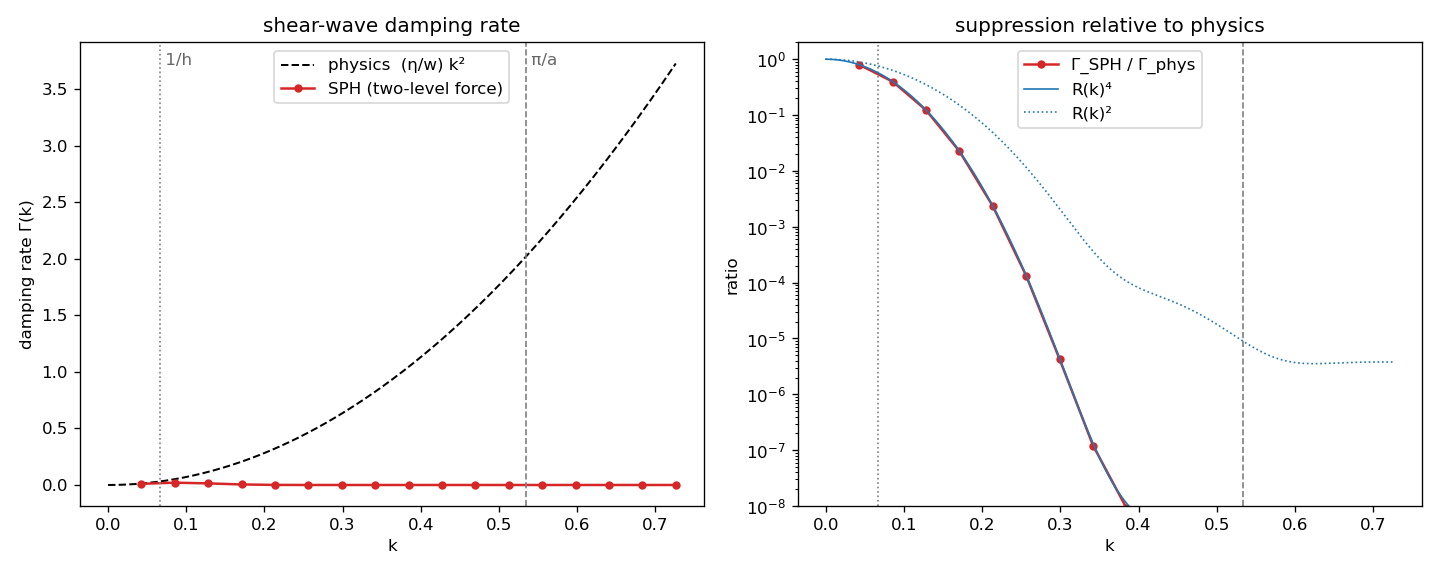
\includegraphics[width=0.9\textwidth]{figs/damping_rate.png}
\caption{Deterministic damping rate of a shear wave on the frozen lattice
(\texttt{damping\_rate.jl}).  Left: $\Gamma(k)$ for the two-level force and the
physical $(\eta/w)k^2$.  Right: the ratio, with $R(k)^4$ and $R(k)^2$.}
\label{fig:damp}
\end{figure}

This measurement has no noise and no time stepping, and it does not start
from rest.  On the frozen lattice put a small shear wave in the momenta,
$m_a=A\,\hat y\cos(kx_a)$ with $A$ chosen so $v\sim10^{-4}$.  Refresh the
fields, evaluate the deterministic two-level force \texttt{dissipative\_force!}
once, and project it onto the wave:
\st
\Gamma_{\rm SPH}(k) = -\frac{\sum_a f_a\cdot m_a}{\sum_a m_a\cdot m_a}\,.
\stp
Since the mean drift of the sweep is this force (\Sect{sec:det}), this is also
the damping rate of the stochastic scheme.  Physically a shear wave decays at
$\Gamma_{\rm phys}=(\eta/w)k^2$, so the shortest waves die fastest.
\Fig{fig:damp} and Table~\ref{tab:damp} show that the scheme does the opposite:
\st
\boxed{\;\Gamma_{\rm SPH}(k) = \Gamma_{\rm phys}(k)\,R(k)^4\;}
\label{eq:R4}
\stp
to three digits for every $k\lesssim0.34$ (beyond that both are below
$10^{-7}$).  The rate peaks near $k\approx0.1$ and then goes to zero.  The four
powers of $R$ have two origins:
\begin{itemize}
  \item $R^2$ \textbf{from the representation}: $\bbeta=\dot x/\Teff$ is built
        from $m$ by two smoothings ($M=\sum m W$, then
        $\dot x_a=\sum_b s_b (v/S)_b W$), so $\bbeta_{\mathbf k}\propto R^2 m_{\mathbf k}$.
  \item $R^2$ \textbf{from the discretization of the dissipative function}:
        the strain \eqref{eq:strain} is a kernel gradient of $\bbeta$
        ($\propto kR$), and the force \eqref{eq:twolevel} is a second kernel
        divergence ($\propto kR$).  This ``gradient of a smoothed gradient''
        Laplacian is a wide stencil, the SPH version of odd--even decoupling.
        A Laplacian built from two centred first differences also fails to
        damp the checkerboard mode.
\end{itemize}

\begin{table}[t]
\centering
\begin{tabular}{ccccc}
$k$ & $2\pi/(kh)$ & $R(k)$ & $\Gamma_{\rm SPH}/\Gamma_{\rm phys}$ & $R(k)^4$ \\ \hline
0.043 & 9.8 & 0.945 & 0.795 & 0.796 \\
0.085 & 4.9 & 0.795 & 0.397 & 0.398 \\
0.171 & 2.5 & 0.388 & $2.2\times10^{-2}$ & $2.3\times10^{-2}$ \\
0.256 & 1.6 & 0.108 & $1.3\times10^{-4}$ & $1.3\times10^{-4}$ \\
0.342 & 1.2 & 0.019 & $1.2\times10^{-7}$ & $1.3\times10^{-7}$
\end{tabular}
\caption{Shear-wave damping on the frozen lattice ($2\pi/(kh)$ is the
wavelength in units of $h$).}
\label{tab:damp}
\end{table}

\paragraph{Consequences.}
\begin{itemize}
  \item \textbf{Deterministic runs are affected too.}  A shear wave with
        wavelength $5h$ decays at $40\%$ of the physical rate, and one with
        $10h$ at $80\%$.  The deterministic shear- and sound-wave validations
        should be rechecked against this before anything is calibrated.
  \item \textbf{Why the stochastic momentum grows.}  The following scalings are
        \emph{derived, not measured}; only the rate is measured.  For a mode
        $\mathbf k$ the noise injected per unit time goes as $k^2R^2$ (the
        kick pattern), the friction rate as $k^2R^4$ \eqref{eq:R4}, and the
        equilibrium amplitude as $\langle|m_{\mathbf k}|^2\rangle\propto1/R^2$
        (its energy cost goes through $M=\sum mW$).  For unresolved modes the
        target is huge and the approach to it is very slow, so they simply keep
        growing.  Note that $K$ sets only the rates: the equilibrium is fixed by
        $\mathbb H$ and $\Sbb$.
  \item \textbf{Relation to \app{app:perbond}.}  The per-bond scheme failed
        through the same mechanism.  Its friction acted through the smoothed
        $\bbeta$, so it was suppressed by $R^2$, while its noise was not
        suppressed, so the runaway was fast.  The two-level move puts in less
        noise ($k^2R^2$), which slows the runaway, but it damps by an
        additional $R^2$.  It is not a remedy.  In \app{app:perbond} the
        claim that ``the strain-based friction acts on what is excited'' is
        false.
\end{itemize}

% ----------------------------------------------------------------------------
\subsection{A one-level (bond) form}
\label{sec:bond}

The two-level $K$ damps unresolved modes as $R^4$, and has an exact null mode
at the zigzag.  A one-level (bond) form squares the differences of $\bbeta$
across neighbouring pairs instead, after subtracting a mean-field rotation and
dilation from each.  It has the same continuum limit, including the full
$\kappa^{ijlm}(v)$ of a moving fluid, conserves momentum and angular momentum,
and has no null mode.  It is derived in \texttt{bond\_dissipation.tex} and
selected with \texttt{params.dissipation = :bond} (or
\texttt{SPH\_DISSIPATION=bond}).  Its damping still levels off at the floor
$\sim R^2$, which comes from $\bbeta$ and not from $K$.  The matching noise is
not implemented yet.

\textbf{No choice of $K$ alone can fix this}, because $K$ is a quadratic form in
$\bbeta$ and $\bbeta$ carries $R^2$.  The particle-level momentum needs its own
thermodynamic force.  That means changing $\mathbb H$ or $\Sbb$: for example
the energy representation with particle entropy $\sum_\ell S(e_\ell,m_\ell)$,
for which concavity gives $S(\underline P(x))\ge\underline S(x)$
(\texttt{sph1.tex}, ``Convexity'').

% ============================================================================
% ============================================================================
\appendix

% ============================================================================
\section{Derivation of the mean drift}
\label{app:drift}

Write the kick to $a$ from its own move as $X=\Delta m_a^i$ and the
accept exponent as $Y=\Delta\Sbb_a$; both are linear in $\xi_a$ with frozen
coefficients, so $(X,Y)$ are jointly Gaussian and mean zero, and
\st
\llangle X\,\min(1,e^{Y})\rrangle
   = \tfrac12\llangle XY\rrangle + O(\sigma^3)
\stp
[split $\min(1,e^Y) = 1 + (e^Y-1)\mathds{1}[Y<0]$ and use
$\llangle XY\,\mathds{1}[Y<0]\rrangle = \tfrac12\llangle XY\rrangle$ for a
mean-zero Gaussian pair; the remainder is $O(\sigma_Y^3)=O(\Delta t^{3/2})$].
With $G_j\equiv\sum_b s_b D_j(x_a,x_b)$ this gives
\st
\label{eq:drift_raw}
\big\langle\Delta m_a^i\big\rangle_{\rm acc}
   = \tfrac12\,\Delta t^2\,\frac{s_a^2}{S_a^{3}}\;
     G_j\,\varepsilon_{lk}(x_a)\,\llangle\xi_a^{ij}\xi_a^{kl}\rrangle
   + O(\xi^3)\,.
\stp
Substitute the covariance \eqref{eq:persite_cov} with index pairs $(ij)$,
$(kl)$,
\st
\llangle\xi_a^{ij}\xi_a^{kl}\rrangle
   = \frac{2\,T_{{\rm rel},a}\,\kappa^{ijkl}\big|_a}{\Delta t\,V_a}\,,
\qquad V_a=\frac{s_a}{S_a}\,,
\stp
and collect the prefactors:
\begin{align}
\big\langle\Delta m_a^i\big\rangle_{\rm acc}
  &= \underbrace{\tfrac12\cdot 2}_{=\,1}\;
     \underbrace{\frac{\Delta t^{2}}{\Delta t}}_{=\,\Delta t}\;
     \underbrace{\frac{s_a^{2}}{S_a^{3}}\cdot\frac{S_a}{s_a}}_{=\,s_a/S_a^{2}}\;
     T_{{\rm rel},a}\,\kappa^{ijkl}\big|_a\,\varepsilon_{lk}(x_a)\;G_j \nn\\[2pt]
  &= \Delta t\;\frac{s_a}{S_a^{2}}\;
     T_{{\rm rel},a}\,\kappa^{ijkl}\big|_a\,\varepsilon_{lk}(x_a)\;G_j\,.
\label{eq:drift_mid}
\end{align}
The Metropolis $\tfrac12$ cancels the FDT $2$, and the $1/V_a$ removes one
power of the particle volume.

Next the index contraction.  In \eqref{eq:drift_mid} the strain carries the
Pass-1 convention $\varepsilon_{lk}=$ (gradient index first, velocity index
second), so $\kappa$'s \emph{last} index $l$ meets the gradient slot and its
\emph{third} index $k$ the velocity slot --- the opposite order from the
deterministic contraction $\kappa^{ijlm}\varepsilon_{lm}$.  One dummy relabel
($k\to m$) and the symmetry of $\kappa$ in its last pair
($\kappa^{ijml}=\kappa^{ijlm}$, true of the $2\eta(\cdots)+\zeta(\cdots)$
structure) fix this:
\st
\kappa^{ijkl}\,\varepsilon_{lk}
   \;\overset{k\to m}{=}\; \kappa^{ijml}\,\varepsilon_{lm}
   \;=\; \kappa^{ijlm}\,\varepsilon_{lm}\,;
\stp
in particular only the \emph{symmetric} part of $\varepsilon$ survives, as in
the deterministic force.  With $G_j$ restored,
\st
\label{eq:drift_Aa}
\big\langle\Delta m_a^i\big\rangle_{\rm acc}
   = \Delta t\;\frac{s_a}{S_a^{2}}\;
     \big(T_{\rm rel}\kappa^{ijlm}\big|_a\,\varepsilon_{lm}(x_a)\big)\,
     \sum_b s_b\,D_j(x_a,x_b)\,,
\stp
precisely the particle-$a$ stress contribution to the two-level force
\eqref{eq:twolevel}.

This is half of the story: \eqref{eq:drift_Aa} is the mean kick $a$ receives
\emph{from its own move}.  But $a$ is also a neighbour of each $b$, so it is
kicked again --- in reaction --- every time $b$ does \emph{its} move.  Bond
$(b,a)$ is one of $b$'s bonds, so $b$'s move applies
\st
\Delta m_a \mathrel{-}= \Delta t\,\frac{s_a s_b}{S_b^{2}}\,
   \xi_b^{ij}\,D_j(x_b,x_a)
 \;=\; +\,\Delta t\,\frac{s_a s_b}{S_b^{2}}\,\xi_b^{ij}\,D_j(x_a,x_b)
\stp
(kernel antisymmetry), and this kick is accepted with \emph{b's} exponent
$\Delta\Sbb_b=\Delta t\,V_b\,\xi_b^{kl}\varepsilon_{lk}(x_b)$ --- the same
$\xi_b$ in both, so \eqref{eq:drift_raw}--\eqref{eq:drift_Aa} go through with
every coefficient evaluated at $b$:
\st
\big\langle\Delta m_a^i\big\rangle_{\rm acc}^{(b\text{'s move})}
   = \Delta t\;s_a s_b\,D_j(x_a,x_b)\;
     \frac{T_{\rm rel}\kappa^{ijlm}\big|_b\,\varepsilon_{lm}(x_b)}{S_b^{2}}\,.
\stp
The draws $\xi_a$, $\{\xi_b\}$ are independent, so over one full sweep the
means add --- $a$ is touched once as owner and once per neighbour as reactor
--- giving \eqref{eq:drift_full}.

% ============================================================================
\section{Sweep order, parallelism, and exactness}
\label{app:sweep}

With the coefficient freeze and the accumulator fields --- no in-place update
of $m,s$ --- each particle's proposal $\xi_a$, its kicks, and its accept test
depend only on frozen coefficients, the precomputed $\varepsilon_a$, and that
particle's own draws $(\xi_a,U_a)$.  Every particle carries its \textbf{own
Xoshiro stream} $\texttt{rngs}[a]$, a vector of $N$ generators seeded once per
run from a master \texttt{Xoshiro(seed)} (\texttt{seed} from \texttt{SimParams}).
The stream is tied to the particle index, not to when the particle is visited,
and the streams advance from one sweep to the next.  Nothing one move reads is
written by another; the sole inter-move coupling is the additive accumulation
into $(\Delta m,\Delta s)$, which commutes.

\paragraph{Order-independence.}
Because particle $a$ always draws from $\texttt{rngs}[a]$, a single pass yields
the same $(\Delta m,\Delta s)$ regardless of visit order --- fixed,
random-permuted, or fully parallel.  The accepted set and every kick are
\emph{bit-identical} across orderings; the per-particle sums differ only by
floating-point associativity ($\sim$ a few ulps).

\paragraph{One move per particle.}
Every particle is visited exactly once per sweep, so the noise/dissipation dose
per $\Delta t$ is spatially uniform by construction.  Non-uniform density
needs no attempt-weight correction: the covariance \eqref{eq:persite_cov}
carries $1/V_a$ and the strain \eqref{eq:strain} carries $1/S_a$, so the
density dependence is exactly that of the deterministic force.

\paragraph{Synchronous (parallel) sweep.}
Decoupled decisions $+$ additive writes: propose and decide all particles in
parallel; reduce the accepted kicks (atomics or per-thread partials); apply.
The per-particle stream vector makes every kick and accept flag independent of
thread/rank count (particle $a$'s noise is fixed no matter which thread runs
its move); only the reduction order (the last few ulps) changes.  Distributed
memory: standard MD halo --- exchange positions and frozen coefficients within
$2h$ of each subdomain boundary (the strain pass needs $\bbeta$ within $2h$;
the kicks reach $2h$), compute owned particles, reduce boundary contributions to
owners.

\paragraph{Exactness: Metropolis-within-Gibbs.}
The frozen synchronous sweep is \emph{not} an exact sampler of $e^{\Sbb}$:
each particle's accept test ignores the kicks applied by the other moves in the
same sweep (their stencils overlap within $2h$), so the composite kernel
preserves $e^{\Sbb}$ only up to the standard $O(\Delta t)$ weak
(Euler--Maruyama-type) error.  The classical exact alternative is
\emph{sequential Metropolis-within-Gibbs}: visit particles in order, fold each
accepted move into the live state and refresh $\bbeta_c$ of the touched
particles before the next move --- each single-particle kernel then satisfies detailed
balance and the composite preserves the target.  But even this is exact only
if the state dependence of the proposal covariance \eqref{eq:persite_cov}
($T_{{\rm rel},a}$, $\kappa(v_a)$, $V_a$ all move with the state) is included
through the Gaussian Hastings ratio; dropping it is again an $O(\Delta t)$
bias (the usual multiplicative-noise ambiguity).  Since \emph{both} variants
carry $O(\Delta t)$ weak bias, the frozen sweep --- fully parallel and
order-independent --- loses nothing in accuracy order; the sequential $+$
Hastings variant is the recorded upgrade path if precision equilibrium
statistics are ever needed.

% ============================================================================
\section{Known biases and their sizes}
\label{app:accuracy}

None of the following affects the sound-wave decay target at leading order;
they are recorded so the diagnostics test for the \emph{expected} deviations.

\paragraph{(a) Stationary distribution: $O(\Delta t)$ weak bias.}
From the coefficient freeze (\app{app:sweep}).  Affects equilibrium
fluctuation amplitudes at $O(\Delta t)$, not the mean drift.  Detect by
running the equilibrium test at $\Delta t$ and $\Delta t/2$; cure, if ever
needed, by sequential Metropolis-within-Gibbs with the Hastings ratio.

\paragraph{(b) Energy bookkeeping: the linearized $\Delta s$ heats at
$O(1/s_a)$.}
\Eq{eq:ds} is the \emph{first-order} term of ``choose $\Delta s$ so that
$\mathbb H$ is conserved'':
\st
\Delta\mathbb H
 = \underbrace{\dot x_c\cdot\Delta m_c + \Teff_c\,\Delta s_c}_{=\,0}
 \;+\; \tfrac12\,\Delta m\cdot\frac{\partial^2\mathbb H}{\partial m^2}
 \cdot\Delta m + \dots
\stp
Deterministically $\Delta m\sim\Delta t$ and the dropped term is a harmless
$O(\Delta t^2)$ --- which is why \texttt{dissipative\_step!} gets away with
the same formula.  Stochastically $\Delta m\sim\sqrt{\Delta t}$, so the
dropped term is $O(\Delta t)$ per step and \emph{sign-definite} (positive
kinetic Hessian): every landed kick heats by $\sim\Delta m^2/2m_{\rm eff}$,
which summed is the FDT noise-injection power.  The friction work is booked
into $s$ correctly; the noise heating is booked nowhere, so $\mathbb H$
drifts monotonically upward at the relative rate
\st
\frac{\dot{\mathbb H}}{\mathbb H}\;\sim\;\frac{1}{s_a\,\tau_{\rm visc}}\,,
\stp
suppressed by the per-particle entropy $s_a\gtrsim10^3$.  Treat
$\Delta\mathbb H(t)$ as an \emph{expected-drift diagnostic}: small, positive,
linear in $t$, with this rate --- its magnitude is itself a check of the
noise normalization.  Upgrade if ever needed: midpoint evaluation
$\Delta s_c = -\tfrac12[\bbeta_c(m)+\bbeta_c(m+\Delta m)]\cdot\Delta m_c$
(residual $O(\Delta m^3)$), at the cost of a velocity re-solve per accepted
move.  The mean drift \eqref{eq:drift_full} is unaffected: a quadratic
addition to $\Delta\Sbb_a$ shifts the Metropolis mean only through vanishing
Gaussian third moments.

\paragraph{(c) The realized increments are non-Gaussian --- by design.}
The accepted kick distribution is the Gaussian proposal \emph{tilted} by the
acceptance: in the scalar toy ($\Delta\Sbb=c\,\xi$, $\xi\sim N(0,\sigma^2)$)
it is the untouched Gaussian on the favorable side, a Gaussian \emph{shifted}
to $c\sigma^2$ on the unfavorable side ($N(\xi)e^{c\xi}\propto
e^{-(\xi-c\sigma^2)^2/2\sigma^2}$), plus a rejection point mass at zero.  Its
mean $\tfrac12 c\sigma^2$ \emph{is} the drift --- the tilt cannot be removed
without removing the dissipation.  Higher cumulants are $O(\Delta t^{3/2})$
and vanish in the diffusion limit.  Additionally, the linearized
$\Delta\Sbb_a$ mis-weights rare large kicks by $e^{O(k^2\Delta t/\tau)}$ at
$k$ standard deviations, distorting only far tails
($k\sim\sqrt{\tau/\Delta t}$) that are never sampled.  Only mean and
covariance survive at $O(\Delta t)$ --- both are exactly right by
\Sect{sec:det}.

% ============================================================================
\section{Why not per-bond accept/reject (record)}
\label{app:perbond}

The first design used one Metropolis test per \emph{bond}: a pair kick
$\delta_{ab}\propto\Delta t\,\mathcal A\sqrt{s_as_b}\,(\xi_a/S_a+\xi_b/S_b)
D(a,b)$ accepted with $\min(1,e^{-(\bbeta_a-\bbeta_b)\cdot\delta_{ab}})$.  It
was coded, tested, and deleted --- it fails structurally; do not revisit:
\begin{itemize}
  \item \textbf{The mean is the single-level force, always.}  The accept
        probability sees only $\delta_{ab}$, so
        $\llangle\delta_{ab}\rrangle_{\rm acc}\propto
        \llangle\delta_{ab}\delta_{ab}\rrangle\,\Delta\bbeta^{(ab)}$ is a
        single-bond object with \emph{coincident} kernel gradients
        $D_j(a,b)D_l(a,b)$ --- never the two-level strain.  No prefactor
        choice changes this.
  \item \textbf{The single-level force is dimensionally $1/{\rm vol}$ too
        big:} $D_l(a,b)\,\Delta\bbeta^{(ab)}$ is not a gradient estimator
        ($\sim[T^2]$ where $\partial_l\bbeta$ is dimensionless); the
        amplitude $\mathcal A$ had to absorb a volume factor and be
        calibrated.
  \item \textbf{Odd-even runaway.}  On a quiescent uniform background the
        per-bond kicks inject independent grid-scale momentum that the
        \emph{smoothed} $\bbeta_a$ cannot see, so the accept/reject provides
        no friction on those modes: $\mathrm{rms}(m_a)\propto\sqrt{t}$
        without bound at every amplitude (observed), while the resolved
        (smoothed) sector stayed flat.
\end{itemize}
The per-particle move fixes all three at once: the accept test sees the full
strain $\varepsilon_a$ [\eqref{eq:dSa}], the mean is the two-level force with
the volume power correct (\app{app:drift}), and the injected pattern
$\xi_a\,D(x_a,x_b)$ is smooth in $b$ (a kernel-gradient dipole), so the
grid-scale modes are excited far less and the strain-based friction acts on
what is excited.

\paragraph{Correction (see \Sect{sec:results}).}
The last claim is false.  The friction on a mode $\mathbf k$ is
$\Gamma_{\rm phys}R(k)^4$ (measured, \Fig{fig:damp}).  Two powers of $R$ come
from the smoothed $\bbeta$, which the per-bond scheme shared, and two come from
the wide two-level stencil.  The per-particle move suppresses the noise in
those modes, which slows the runaway, but suppresses the friction even more.
The per-particle sweep still shows the per-bond symptom (resolved sector flat,
unresolved momentum growing), only more slowly.

% ============================================================================
\section{Implementation}
\label{app:impl}

Reused unchanged: \texttt{sph.jl} (\texttt{Particle}, EOS,
\texttt{kappa\_tensor}), \texttt{celllist.jl} (\texttt{leapfrog\_step!},
cell-list machinery, \texttt{dissipative\_force!} Pass~1,
\texttt{wendland\_c2\_grad}, \texttt{minimum\_image}), \texttt{setup.jl} (IC
helpers, \texttt{thermalize!}), \texttt{io.jl} (\texttt{SnapshotWriter}).
New code lives in \texttt{stochastic.jl} $+$ driver scripts.

\paragraph{Noise draw in code.}
\texttt{generate\_noise} (\texttt{sph2.tex} App.~E1) returns the
unit-normalized stress $\hat\xi$ with
$\llangle\hat\xi^{ij}\hat\xi^{lm}\rrangle=\kappa^{ijlm}(v)$ (\emph{no}
$T_{\rm rel}$); \texttt{draw\_xi} rescales by $\sqrt{2T_{\rm rel}}$ to the
continuum FDT normalization $2\,\texttt{kappa\_tensor}$ (verified by MC
audit, \texttt{teststochastic.jl} Step~2, at all $v$).  The per-particle draw of
\eqref{eq:persite_cov} is then $\texttt{draw\_xi}/\sqrt{\Delta t\,V_a}$.

\paragraph{The full loop.}
\begin{enumerate}
  \item IC: uniform background, small periodic box (\texttt{setup\_ic} /
        \texttt{setup\_shear\_wave}); \texttt{thermalize!}.
  \item Per step: \texttt{leapfrog\_step!} $\to$ \texttt{rebuild\_cell\_list!}
        $\to$ refresh$+$freeze (\texttt{smooth\_to\_particles!},
        \texttt{update\_thermodynamics!}, \texttt{update\_velocities!}) $\to$
        strain pass $\to$ \texttt{particle\_sweep!} $\to$
        \texttt{apply\_sweep!} $\to$ diagnostics.
\end{enumerate}

\paragraph{Status.}
Done: accumulator fields $+$ \texttt{apply\_sweep!} (Step~0); the cell-list
neighbour stencil --- the traversal used by the strain pass and the sweep ---
validated against $O(N^2)$ brute force (Step~1; requires
$\texttt{ncx},\texttt{ncy}\ge3$); \texttt{draw\_xi} $+$ MC covariance audit
(Step~2).  The per-bond sweep and its bond list were coded, tested, and
deleted (\app{app:perbond}).

\paragraph{Step 3: \texttt{particle\_sweep!}.}
\begin{lstlisting}
particle_sweep!(particles, params, cl, eos, dt, rngs=PHYS_RNG) -> (n_acc, n_try, ΔS_tot)
  # coefficients frozen; ε_a from the strain pass (dissipative_force! Pass 1)
  # rngs[a] : particle a's own Xoshiro (rng.jl), seeded once per run
  for a in eachindex(particles); particles[a].Δm = 0; particles[a].Δs = 0; end
  for a in eachindex(particles)
      rng = rngs[a]
      Va  = particles[a].s / particles[a].S_smooth
      ξa  = draw_xi(rng, particles[a], eos, cs2v) / sqrt(dt * Va)   # cov: eq (persite_cov)
      ΔS  = dt * Va * sum(ξa[i,j]*ε_a[j,i] for i,j)         # = dt V_a ξ:ε   eq (dSa)
      n_try += 1
      if rand(rng) < exp(ΔS)                               # test BEFORE bond loop
          for b in neighbors(a), r_ab < 2h                 # cell-list stencil
              grad = wendland_c2_grad(x_a - x_b, ...)
              f    = dt * (s_a*s_b / S_a^2) * (ξa * grad)  # SVector{2}     eq (kicks)
              particles[a].Δm += f ; particles[a].Δs -= dot(b_vec[a], f)
              particles[b].Δm -= f ; particles[b].Δs += dot(b_vec[b], f)
          end
          n_acc += 1 ; ΔS_tot += ΔS
      end
  end
\end{lstlisting}
The accumulators are zeroed at entry (a full pass first --- a particle is
written as a neighbour of others' moves), so no caller-side reset is needed;
\texttt{apply\_sweep!} folds $(\Delta m,\Delta s)$ into $(m,s)$ afterwards.
The accept test needs only $\xi_a$ and $\varepsilon_a$ [\eqref{eq:dSa}] --- no
neighbour loop --- so rejected proposals cost $O(1)$.
\emph{Checks} (extend \texttt{teststochastic.jl}):
(i) $\eta/s=0\Rightarrow$ all $\Delta m,\Delta s=0$;
(ii) $|\sum_a\Delta m_a|/\sum_a|\Delta m_a|<10^{-12}$;
(iii) GENERIC degeneracy
$\sum_a(\Teff_a\Delta s_a+\dot x_a\cdot\Delta m_a)=0$ to round-off;
(iv) per-particle stream vector $\Rightarrow$ visit-order independence
(shuffled particle order reproduces $(\Delta m,\Delta s)$ to $<10^{-12}$);
(v) the identity \eqref{eq:dSa}: the cheap
$\Delta t V_a\,\xi\!:\!\varepsilon$ equals the explicit
$-\sum_c\bbeta_c\cdot\Delta m_c$ over the distributed kicks, per particle, to
round-off;
(vi) \textbf{mean drift:} many sweeps on one frozen sheared state,
$\langle\Delta m_a\rangle/\Delta t$ vs.\ \texttt{dissipative\_force!} ---
slope~1, the decisive test of \eqref{eq:drift_full}.

\paragraph{Then.}
\emph{Uniform-background stability} (\texttt{teststochastic\_run.jl} rewired):
$s_a\gtrsim10^3$; $\mathrm{rms}(m_a)$ saturates at the FDT value;
$\mathbb H$ drift positive at the \app{app:accuracy}(b) rate; acceptance
$\gtrsim0.99$; repeat at $\Delta t/2$.
\emph{Shear-wave validation} (\texttt{teststochastic\_shear.jl}):
ensemble-averaged decay of $M^y=A\sin(kx)$ vs.\ $(\eta/s)k^2/T_0$, no tuned
parameter; an $\eta/s=0$ run measures the numerical baseline.
\emph{2D sound-wave decay --- the target}
(\texttt{teststochastic\_sound.jl}, built on \texttt{testsound\_viscous.jl}):
eigenmode IC with genuinely 2D $\vec k$ ($n_x=n_y=1$); ensemble-mean
amplitude decay vs.\ $e^{-\Gamma_s k^2t/2}$,
$\Gamma_s=(\tfrac43\eta/s+\zeta/s)/T_{{\rm rel},0}$; final profile vs.\
\texttt{analytic\_M}; no fitting.
\emph{Parallel sweep} (optional): parallel particle loop, reduction into the
accumulators; bit-identical to serial for the same key (\app{app:sweep}).

\begin{thebibliography}{9}
% TODO
\end{thebibliography}

\end{document}
